\documentclass{article}
\usepackage{amsmath}
\usepackage{tikz}
\usepackage{pgfplots}
\pgfplotsset{compat=1.16}

\begin{document}

\begin{figure}[h]
    \centering
    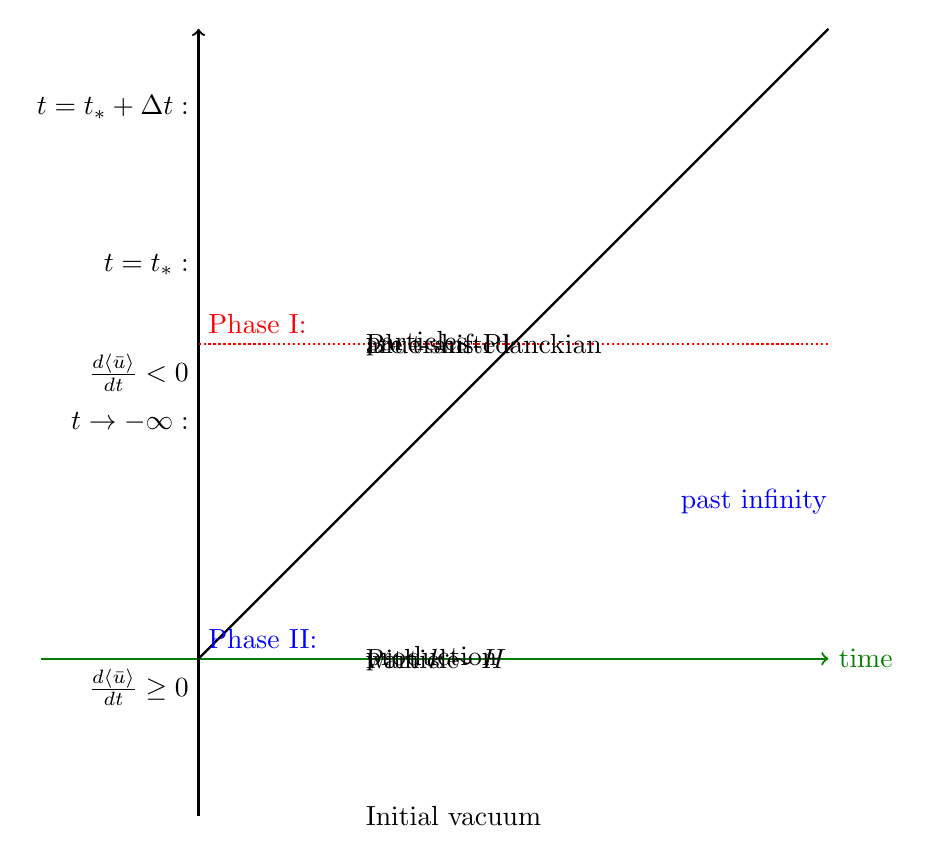
\begin{tikzpicture}
        % Draw the vertical axis
        \draw[->, green!50!black, thick] (-2, 0) -- (8, 0) node[right] {time};
        
        % Draw the horizontal axis
        \draw[->, black, thick] (0, -2) -- (0, 8);
        
        % Draw the red line for Phase I
        \draw[red, densely dotted, thick] (0, 4) -- (8, 4);
        
        % Draw the black line for Phase II
        \draw[black, thick] (0, 0) -- (8, 8);
        
        % Annotate the lines
        \node at (0, 4) [above right] {\textcolor{red}{Phase I:}};
        \node at (0, 4) [below left] {$\frac{d\left<\bar{u}\right>}{dt} < 0$};
        
        \node at (0, 0) [above right] {\textcolor{blue}{Phase II:}};
        \node at (0, 0) [below left] {$\frac{d\left<\bar{u}\right>}{dt} \geq 0$};
        
        % Annotate the time labels
        \node at (0, 7) [left] {$t = t_* + \Delta t:$};
        \node at (0, 5) [left] {$t = t_*:$};
        \node at (0, 3) [left] {$t \rightarrow -\infty:$};
        
        % Annotate the text for Phase I
        \node at (2, 4) [right] {\textcolor{black}{Blue-shifted}};
        \node at (2, 4) [right] {\textcolor{black}{particles}};
        \node at (2, 4) [right] {\textcolor{black}{are trans-Planckian}};
        
        % Annotate the text for Phase II
        \node at (2, 0) [right] {\textcolor{black}{Particle}};
        \node at (2, 0) [right] {\textcolor{black}{production}};
        \node at (2, 0) [right] {\textcolor{black}{with $k \sim H$}};
        
        % Annotate the text for initial vacuum
        \node at (2, -2) [right] {\textcolor{black}{Initial vacuum}};
        
        % Annotate the text for past infinity
        \node at (6, 2) [right] {\textcolor{blue}{past infinity}};
    \end{tikzpicture}
    \caption{The Penrose diagram of the CPT conjugated of the TCC-violating expanding solution that satisfies our assumptions. If we start with the past vacuum state, there will be particle production at the moment of transition from Phase II to Phase I. Under our assumptions, Phase I lasts long enough to blue-shift those particles to trans-Planckian energies that violate the EFT.}
    \label{fig:penrose_diagram}
\end{figure}

\end{document}